% ----------------------- TODO ---------------------------
% Change per hand-in
\newcommand{\NUMBER}{1} % exercise set number
\newcommand{\EXERCISES}{5} % number of exercises

\newcommand{\COURSECODE}{AP3252}
\newcommand{\TITLE}{Condensor System}
\newcommand{\STUDENTA}{Jeroen Sangers}
\newcommand{\DEADLINE}{DEADLINE}
\newcommand{\COURSENAME}{Electron Microscopy: Characterisation of the nanoscale}
% ----------------------- TODO ---------------------------

\documentclass[a4paper]{scrartcl}

\usepackage[utf8]{inputenc}
\usepackage[british]{babel}
\usepackage{amsmath}
\usepackage{amssymb}
\usepackage{fancyhdr}
\usepackage{color}
\usepackage{graphicx}
\usepackage{lastpage}
\usepackage{listings}
\usepackage{tikz}
\usepackage{pdflscape}
\usepackage{subfigure}
\usepackage{float}
\usepackage{polynom}
\usepackage{hyperref}
\usepackage{tabularx}
\usepackage{forloop}
\usepackage{geometry}
\usepackage{listings}
\usepackage{fancybox}
\usepackage{tikz}
\usepackage{algpseudocode,algorithm,algorithmicx}
\usepackage{fontspec}
\setmainfont{Baskerville Light}[
	BoldFont	= Baskerville Bold ,
	ItalicFont	= Baskerville Light-Italic
]


% Algorithm command
\newcommand*\Let[2]{\State #1 $\gets$ #2}

% Matrix notation
\newcommand{\matr}[1]{\mathbf{#1}}

% Margins
\geometry{a4paper,left=3cm, right=3cm, top=3cm, bottom=3cm}

% Header and footer setup
\pagestyle {fancy}
%\fancyhead[L]{Tutor: \TUTOR}
\fancyhead[L]{\TITLE}
\fancyhead[C]{\STUDENTA}
\fancyhead[R]{\today}

\fancyfoot[L]{\COURSECODE}
\fancyfoot[C]{\COURSENAME}
\fancyfoot[R]{Page \thepage /\pageref*{LastPage}}

% Formatting of "title"
\def\header#1#2{
  \begin{center}
    {\Large Exercise set}\\
    {(Deadline #2)}
  \end{center}
}

\begin{document}
\subsection*{Exercise 1}

For parallel illumination of the sample the beam crossover after the lens $\mathcal{C}2$ needs to be placed in the focal point of the lens $\mathcal{C}3$.
Keeping the focal point of lens $\mathcal{C}1$ fixed, the focal points of lens $\mathcal{C}2$ and $\mathcal{C}3$ can be changed such that the crossover point after the lens $\mathcal{C}2$ falls in the focal point of $\mathcal{C}3$.

\begin{figure}
  \centering
  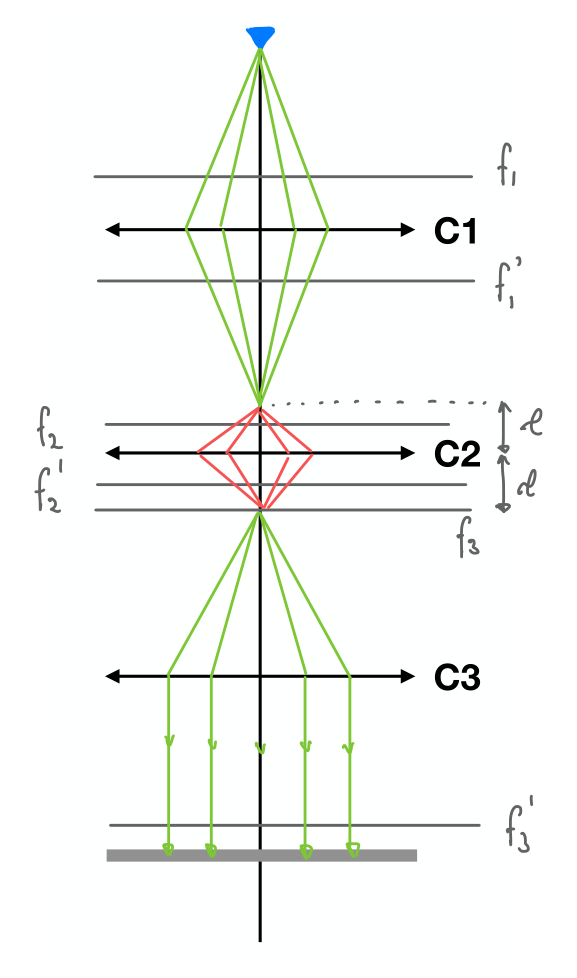
\includegraphics[width=.5\textwidth, keepaspectratio]{fig.png}
\end{figure}

\end{document}